\documentclass[tikz,border=5mm]{standalone}
\usetikzlibrary{decorations.markings}

\begin{document}
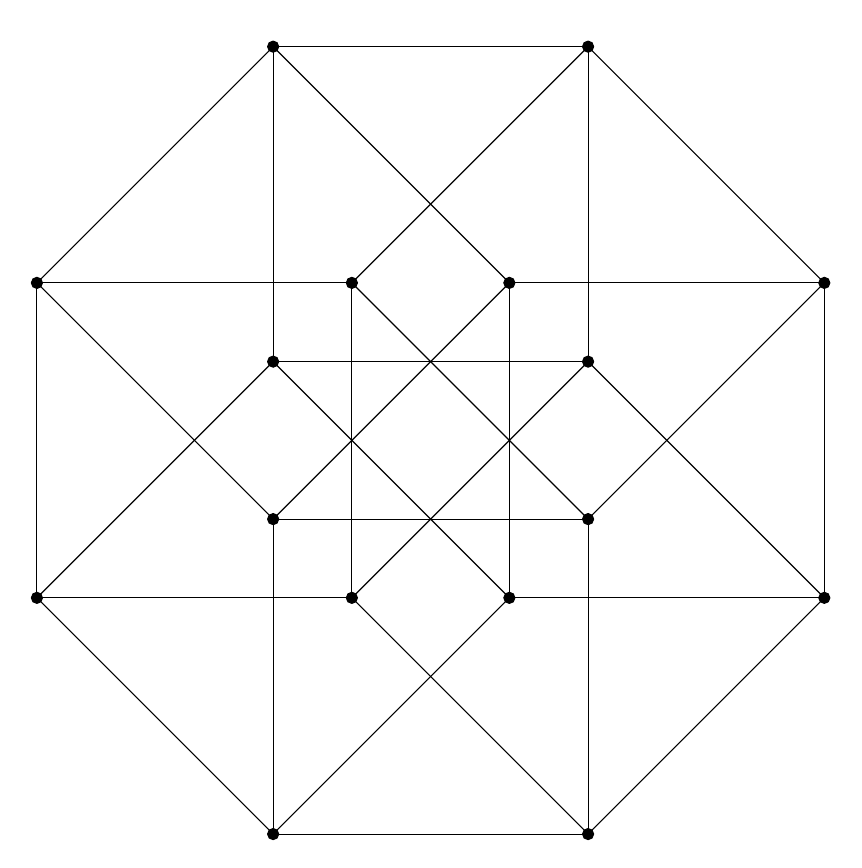
\begin{tikzpicture}[every loop/.style={min distance=30mm}]

    % these are the vertices
    \draw[fill=black] (20, 20) circle (2pt) node[above] {};
    \draw[fill=black] (24, 20) circle (2pt) node[above] {};
    \draw[fill=black] (20, 16) circle (2pt) node[above] {};
    \draw[fill=black] (24, 16) circle (2pt) node[above] {};

    \draw[fill=black] (20, 14) circle (2pt) node[above] {};
    \draw[fill=black] (24, 14) circle (2pt) node[above] {};
    \draw[fill=black] (20, 10) circle (2pt) node[above] {};
    \draw[fill=black] (24, 10) circle (2pt) node[above] {};

    \draw[fill=black] (17, 17) circle (2pt) node[above] {};
    \draw[fill=black] (21, 17) circle (2pt) node[above] {};
    \draw[fill=black] (17, 13) circle (2pt) node[above] {};
    \draw[fill=black] (21, 13) circle (2pt) node[above] {};

    \draw[fill=black] (23, 17) circle (2pt) node[above] {};
    \draw[fill=black] (27, 17) circle (2pt) node[above] {};
    \draw[fill=black] (27, 13) circle (2pt) node[above] {};
    \draw[fill=black] (23, 13) circle (2pt) node[above] {};


    \draw (20, 20) -- (24, 20) -- (24, 16) -- (20, 16) -- (20, 20);
    \draw (20, 14) -- (24, 14) -- (24, 10) -- (20, 10) -- (20, 14);
    \draw (17, 17) -- (21, 17) -- (21, 13) -- (17, 13) -- (17, 17);
    \draw (23, 17) -- (27, 17) -- (27, 13) -- (23, 13) -- (23, 17);
    \draw (20, 20) -- (17, 17);
    \draw (17, 13) -- (20, 10);
    \draw (24, 10) -- (27, 13);
    \draw (27, 17) -- (24, 20);
    \draw (20, 20) -- (23, 17);
    \draw (24, 20) -- (21, 17);
    \draw (17, 17) -- (20, 14);
    \draw (17, 13) -- (20, 16);
    \draw (20, 10) -- (23, 13);
    \draw (24, 10) -- (21, 13);
    \draw (27, 17) -- (24, 14);
    \draw (27, 13) -- (24, 16);
    \draw (21, 17) -- (24, 14);
    \draw (23, 17) -- (20, 14);
    \draw (24, 16) -- (21, 13);
    \draw (20, 16) -- (23, 13);

\end{tikzpicture}
\end{document}
